% !TEX TS-program = pdflatex
% !BIB TS-program = biber
\documentclass[12pt,letterpaper]{article}

% Layout and formatting
\usepackage[margin=1in]{geometry}
\usepackage{acronym}
\usepackage{csquotes}
\usepackage{fixltx2e}
\usepackage{url}
\usepackage[T1]{fontenc}
\usepackage{mathptmx}
\usepackage{setspace}
\usepackage{units}
%\usepackage{etoolbox}
%\BeforeBeginEnvironment{equation}{\begin{singlespace}}
%\AfterEndEnvironment{equation}{\end{singlespace}\noindent\ignorespaces}
%\BeforeBeginEnvironment{align}{\begin{singlespace}}
%\AfterEndEnvironment{align}{\end{singlespace}\noindent\ignorespaces}
\frenchspacing

% Graphics
\usepackage{graphicx}
\usepackage[pdf]{pstricks}
\psset{unit=1in,linewidth=0.02,arrows=C-C,arrowsize=0.2}

% Bibliography
\usepackage[american]{babel}
\usepackage[backend=biber,style=apa]{biblatex}
\DeclareLanguageMapping{american}{american-apa}
\bibliography{bibliography.bib}
\newcommand{\aposcite}[2]{\citeauthor{#1}'s #2 (\citeyear{#1})}
\usepackage{doi}

% Figures, tables, and captions
\usepackage{float}
\usepackage{booktabs}
\usepackage[hypcap]{caption}
\captionsetup{labelfont=bf,font=small,labelsep=period}
\usepackage{subcaption}
\usepackage[rightcaption]{sidecap}
\usepackage[plain]{fancyref}

% Math
\usepackage{amsmath}
\usepackage[algoruled]{algorithm2e}
\usepackage{mathtools}
\usepackage{commath}

\newcommand{\R}{\ensuremath{\mathcal{R}}}

\title{Bayesian Reconstruction of Coevolutionary Histories}

% Acronyms
\acrodef{CDF}{cumulative distribution function}
\acrodef{ESS}{estimated sample size}
\acrodef{GMTC}{geographic mosaic theory of coevolution}
\acrodef{GTR}{general time reversible}
\acrodef{MCC}{maximum clade credibility}
\acrodef{MCMC}{Markov chain Monte Carlo}

% Reusable figures
\newcommand{\pscophylogeny}{
\begin{pspicture}(18,12)
\psset{unit=0.5cm,linewidth=0.2}
\psline[linecolor=blue](0,0)(10,10)
\psline[linecolor=blue](4,0)(2,2)
\psline[linecolor=blue](8,0)(4,4)
\psline[linecolor=blue](12,0)(14,2)
\psline[linecolor=blue](16,0)(8,8)
\psline[linecolor=red](1,0)(11,10)
\psline[linecolor=red,arrows=-o](17,0)(9,8)
\psline[linecolor=red,arrows=-o](13,0)(15,2)
\psline[linecolor=red](7,3)(14,3)
\psline[linecolor=red,arrows=<-](10,3)(14,3)
\psline[linecolor=red](10,0)(7,3)
\psline[linecolor=red,arrows=-o](9,0)(5,4)
\psline[linecolor=red,arrows=-o](4,1)(3,2)
\rput{135}(4,1){\LARGE\textcolor{red}{\textsf{\textbf{x}}}}
\psline[linecolor=red](18,0)(17,1)
\psline[linecolor=red,arrows=*-](16,1)(17,1)
\end{pspicture}
}

\begin{document}

\begin{titlepage}
\null
\vfil
\let\newpage\relax
\maketitle
\vfil
\centering
\pscophylogeny
\vfil
\thispagestyle{empty}
\end{titlepage}

\newpage

\doublespacing

\section*{Introduction}

Organismic symbioses, or interactions between individuals of two or more different species, constitute a fundamental aspect of many living systems and occur across the biological spectrum. The characteristics of symbiotic relationships can vary greatly, particularly in degrees of cooperation (parasitism vs. mutualism), fidelity (generalized vs. specialized and species-specific), and obligation (optional vs. vital to survival) \parencites{Herre:1999}{Charleston:2002}{Oberprieler:2004}{Machado:2005}{Becerra:2007}{Beinart:2012}{HoyalCuthill:2012}{Thompson:2012}{Faria:2013}. Understanding how these relationships evolve and, in particular, how symbionts affect their partners' evolution---that is, the coevolutionary processes driven by symbiotic interactions---remain important questions in ecology and evolutionary biology.

Phylogenies, or evolutionary trees, can provide a valuable perspective to evolutionary processes. A species tree is one example of a phylogeny, where its topology depicts the series of speciation events that gave rise to a set of taxa and thus their ancestral relationships \parencite{Baum:2008}. Often, the lengths of branches indicate the number of substitutions (e.g., genetic mutations) accumulated at a lineage or the amount of time that the lineage existed \parencite{Baum:2008}. By mapping traits such as physical attributes or geographic locations onto a known phylogeny, we can use the tree to learn about the mechanisms under which these traits change \parencites{Lemey:2009}{Lemey:2010}{Segraves:2010}.

Molecular sequences are the primary source of data for constructing phylogenies \parencite{Baum:2008}. With the advancements of DNA sequencing technology over the last few decades, considerable effort has been invested in developing methods for inferring phylogenies from sequence alignments (of both nucleotides and amino acids) \parencite{Felsenstein:2005}. One of the first techniques for phylogenetic inference optimized the tree topology under the parsimony criterion \parencite{Fitch:1971}. The most parsimonious tree is the \enquote{simplest} possible explanation for the  sequence alignment: the tree involving the least number of substitution events. However, \textcite{Felsenstein:1978} demonstrated cases in which the parsimony criterion fails to return the correct tree (e.g., when substitution rates vary between lineages, causing a phenomenon he denoted \enquote{long branch attraction}). Following his criticism of parsimony methods, \textcite{Felsenstein:1981} introduced an algorithm to calculate the likelihood of a tree given a sequence alignment and a substitution model. Similar to maximum parsimony, maximum likelihood techniques optimize a tree under \aposcite{Felsenstein:1981}{likelihood function}, often simultaneously estimating parameter values for the substitution model \parencite{Felsenstein:2005}. Likelihood methods can be used with sophisticated substitution models, such as models that consider the underlying molecular processes of evolution \parencite[e.g.,][]{Hasegawa:1985}.

Many recent advances in phylogenetics have focused on methodologies utilizing Bayesian inference \parencites{Huelsenbeck:2001a}{Drummond:2002}. Bayesian inference takes its name from Bayes' theorem \parencite{Bayes:1763} and relies on the principle that the posterior probability of a model's parameters~$\theta$ given some fixed data~$D$ $P\left(\theta\mid D\right)$ is proportional to $P\left(D\mid \theta\right) P\left(\theta\right)$. The likelihood, $P\left(D\mid \theta\right)$, is the probability of observing the data under the model parameters (e.g., \citeauthor{Felsenstein:1981}'s \citeyear{Felsenstein:1981} algorithm), and the prior, $P\left(\theta\right)$, is the probability of the model parameters without considering the data. The prior can be a mechanism to apply previous knowledge to a new analysis; for example, constructing a prior distribution on the mutation rate parameter that is representative of the rates reported in previous literature will \enquote{bias} the posterior to favor those rates. When explicit prior knowledge is not available, an uninformative prior may be applied.

Often we are interested in only some of the parameters involved in an analysis (e.g., just the tree topology), in which case we can calculate the posterior probability of specific values for those parameters by integrating over all possible values of the remaining \enquote{nuisance} parameters (branch lengths, mutation rate, etc.). Due to the complexity of the models, the resulting multi-dimensional integral cannot be evaluated directly but instead approximated via a \ac{MCMC}. Under the Metropolis--Hastings \ac{MCMC} algorithm, the chain advances from one state, or set of parameter values, to the next by randomly mutating the current state and accepting or rejecting this proposal based on its posterior probability \parencites{Metropolis:1953}{Hastings:1970}. With a chain of enough length, the collection of states sampled by the \ac{MCMC} is an approximation of the posterior distribution. Although there have been criticisms of Bayesian \ac{MCMC} methodologies in phylogenetics \parencites{Felsenstein:2005}{Kolaczkowski:2009}, they remain popular for their flexibility, particularly their ability to adopt complex evolutionary models and integrate over uncertainties \parencites{Huelsenbeck:2001b}{Drummond:2007}{Ronquist:2012}.

\textcite{Haffner:1988} were the first to apply phylogenetic methods to study coevolution. After constructing phylogenies for pocket gophers and their parasitic lice, they presented them side-by-side for comparison. Although the speciation patterns between the two trees showed significant similarities, they were not identical, which leads to an important observation: that host--symbiont phylogenies generally do not mirror each other perfectly, even in highly-specialized, obligatory mutualisms \parencite{Machado:2005}. Therefore, there must be more complex processes determining when a symbiont speciates and which hosts its descendants partner with than simple cospeciation, in which the host and symbiont speciate simultaneously and their respective descendants continue the association. As with many other biological processes, we can learn about this coevolutionary process by mapping the set of hosts and their ancestors onto the symbiont tree.

\begin{SCfigure}
\centering
\begin{pspicture}(18,12)
\psset{unit=0.5cm,linewidth=0.2}
\psline[linecolor=blue](0,0)(10,10)
\psline[linecolor=blue](4,0)(2,2)
\psline[linecolor=blue](8,0)(4,4)
\psline[linecolor=blue](12,0)(14,2)
\psline[linecolor=blue](16,0)(8,8)
\psline[linecolor=red](1,0)(11,10)
\psline[linecolor=red,arrows=-o](17,0)(9,8)
\psline[linecolor=red,arrows=-o](13,0)(15,2)
\psline[linecolor=red](7,3)(14,3)
\psline[linecolor=red,arrows=<-](10,3)(14,3)
\psline[linecolor=red](10,0)(7,3)
\psline[linecolor=red,arrows=-o](9,0)(5,4)
\psline[linecolor=red,arrows=-o](4,1)(3,2)
\rput{135}(4,1){\LARGE\textcolor{red}{\textsf{\textbf{x}}}}
\psline[linecolor=red](18,0)(17,1)
\psline[linecolor=red,arrows=*-](16,1)(17,1)
\rput(6,4){\textbf{(a)}}
\rput(16.5,1.5){\textbf{(b)}}
\rput(10,4){\textbf{(c)}}
\rput(5,0.5){\textbf{(d)}}
\end{pspicture}
\caption{An example of a coevolutionary history, with the host phylogeny in blue, the symbiont phylogeny in red, and symbols and letters corresponding with the four events depicted in \Fref{fig:events}. A given symbiont lineage is partnered with the }
\label{fig:cophylogeny}
\end{SCfigure}

An example of such a mapping is provided in \Fref{fig:cophylogeny}. To explain the ancestral associations between the two phylogenies, we rely on a set of coevolutionary events \parencite{Page:2003}: cospeciation, in which the symbiont speciates when its host speciates and one of the new symbiont lineages follows one of the new host lineages and the other symbiont lineage follows the other host lineage; duplication, in which the symbiont speciates independently of the host and both new symbiont lineages remain associated with the same host; host-switch, in which the symbiont speciates independently of the host and one of the new symbiont lineages partners with a new host while the other symbiont lineage remains on the same host; and loss, in which a symbiont lineage goes extinct independently of its host (see \Fref{fig:events}). Any of these events, save cospeciation, can happen independent of the host's evolution, and thus they can occur at any point along the branch of the host. Cospeciation, however, can occur only when the host speciates. Determining the mapping between two trees is denoted the cophylogeny reconciliation problem. Thus, to reconstruct a complete coevolutionary history between a host and a symbiont, we must reconstruct both their phylogenies and reconcile the association between their nodes. Determining the reconciliation implicitly reconstructs the events that created it.

\begin{figure}
\centering
\begin{subfigure}[b]{0.2\textwidth}
\centering
\begin{pspicture}(1,1)
\psline[linecolor=blue](0,0.5)(0.5,0.5)
\psline[linecolor=blue](0.5,0.3)(1,0.3)
\psline[linecolor=blue](0.5,0.7)(1,0.7)
\psline[linecolor=blue](0.5,0.3)(0.5,0.7)
\psline[linecolor=red](0.4,0.4)(1,0.4)
\psline[linecolor=red](0.4,0.8)(1,0.8)
\psline[linecolor=red](0.4,0.4)(0.4,0.8)
\psline[linecolor=red,arrows=-o](0,0.6)(0.4,0.6)
\end{pspicture}
\caption{cospeciation}
\end{subfigure}
\begin{subfigure}[b]{0.2\textwidth}
\centering
\begin{pspicture}(1,1)
\psline[linecolor=blue](0,0)(1,0)
\psline[linecolor=red](0,0.1)(1,0.1)
\psline[linecolor=red,arrows=*-](0.5,0.1)(0.5,0.3)
\psline[linecolor=red](0.5,0.3)(1,0.3)
\end{pspicture}
\caption{duplication}
\end{subfigure}
\begin{subfigure}[b]{0.2\textwidth}
\centering
\begin{pspicture}(1,1)
\psline[linecolor=blue](0,0)(1,0)
\psline[linecolor=blue](0,0.4)(1,0.4)
\psline[linecolor=red](0,0.1)(1,0.1)
\psline[linecolor=red](0.5,0.1)(0.5,0.5)
\psline[linecolor=red,arrows=->,arrowsize=0.1](0.5,0.1)(0.5,0.35)
\psline[linecolor=red](0.5,0.5)(1,0.5)
\end{pspicture}
\caption{host-switch}
\end{subfigure}
\begin{subfigure}[b]{0.2\textwidth}
\centering
\begin{pspicture}(1,1)
\psline[linecolor=blue](0,0)(1,0)
\psline[linecolor=red](0,0.1)(0.8,0.1)
\rput(0.8,0.1){\large\textcolor{red}{\textsf{x}}}
\end{pspicture}
\caption{loss}
\end{subfigure}
\caption{Diagrams of the four cophylogenetic events considered in my model, where the host organism's phylogeny is in blue and the symbiont phylogeny in red. All events are branch events (i.e., they can occur at any point along a branch) except cospeciation, which is a nodal event (and thus can occur only when the host speciates).}
\label{fig:events}
\end{figure}

The cophylogeny reconciliation problem is well-studied thanks to its relevance to two fields of biology. Research has revealed that often phylogenies of individual genes do not match perfectly with each other nor with the overall species phylogeny \parencite{Degnan:2009}. The processes resulting in these discrepancies are similar to those involved in coevolution: gene duplication events, gene loss events, and horizontal gene transfer events \parencite{David:2011}. Not surprisingly, there are a number of programs that implement event-based models for maximum parsimony reconciliation of cophylogenies, e.g., Tarzan \parencite{Merkle:2005}, CoRe-PA \parencite{Merkle:2010}, Jane \parencite{Conow:2010}, TreeMap \parencite{Charleston:2011}, AnGST \parencite{David:2011}, and RANGER-DTL \parencite{Bansal:2012}, either to explicitly reconcile the associations between two trees, or to use the reconciliation to infer the phylogeny of one tree with another, known tree. The reconciliation between two trees is determined by giving penalizing scores to each of the events considered in a model, and optimizing the reconciliation under a function that determines the events involved in a particular reconciliation and thus its score.

However, just as phylogeny reconstruction transition from parsimony to likelihood and Bayesian methodologies, the cophylogeny reconstruction problem could benefit from a probabilistic approach. Some of the problems present in maximum parsimony reconciliation are choosing the assignment of penalties to the events \parencite{Merkle:2010} and treatment of multiple, equally parsimonious reconciliations. Furthermore, parsimony implementations generally expect at least one, if not both, tree topologies to be given (that is, assumed to be correct in all regards), as well as the timings of the nodes of the tree if they are considered by the model. However, when phylogenies are reconstructed using Bayesian \ac{MCMC}, a distribution of topologies is returned, including distributions on the node timings. This additional information, which may significantly influence a reconciliation (e.g., when a most-parsimonious reconciliation relies on a particular timing that has a low posterior probability), is currently not being utilized. A Bayesian \ac{MCMC} method for reconciliation of cophylogenies could work alongside tree reconstruction, thus being influenced by the posterior probability of the entire model.

The fundamental challenge for developing a probabilistic model for reconciliation is the difficulty of accounting for loss events, because they cannot be observed in the present \parencite{Charleston:2009}: at any point in time, a symbiont may have duplicated on its host or switched to another host but then gone extinct, thus hindering our observation of the event. To account for this phenomenon, we can integrate over all possibilities, but it turns out that this integration is not feasible. While a closed-form integration exists for the simpler duplication-loss problem \parencite{Gernhard:2008} which does not consider host-shift/transfer events, no such closed-form solution has been found for models involving transfer events. Another option would be to let the \ac{MCMC} approximate this integral; however, the infinite number of possibilities would greatly hinder performance of the chain and make the problem computationally intractable.

Despite this challenge, solutions have been proposed to approximate the probability of a reconciliation. \textcite{Huelsenbeck:2000} presented the first such solution, a Bayesian \ac{MCMC} implementation of a simple model that considered only host-switch events; however, it was not developed further. More recently, \textcite{Charleston:2009} described a more complex model for cophylogenies and proposed that branches on the host phylogeny be discretized to approximate the integration of unobserved events, but did not implement it. \textcite{Faria:2013} implement a Bayesian \ac{MCMC} method to analyze viral evolution in the context of its host; however, they treat the host phylogeny as fixed and develop a specific rate matrix to describe a transition of the symbiont from any discrete ancestral host to another (and thus also consider only host-switch events). \textcite{Sjostrand:2013} have implemented a cophylogeny model using discretization similar to \aposcite{Charleston:2009}{proposal}, but in the context of the gene tree--species tree problem, where they assume the species tree to be fixed and treat the reconciliation as a nuisance parameter and integrate it out.

I take a different approach to this problem and describe a cophylogeny model to approximate the likelihood of a cophylogenetic reconstruction by considering only the observed events. I implement my algorithm in a Bayesian framework and evaluate with data simulated under the three event model.

\section*{Materials and Methods}

I consider all phylogenies to be rooted, bifurcating trees. I refer to the set of nodes, or vertices, of a tree $T$ as $V(T)$, its leaves as $L(T) \subset V(T)$, and its internal nodes $I(T) = V(T) \setminus I(T)$. The two children of an internal node $v$ are represented by $\text{left}(v)$ and $\text{right}(v)$, and its parent by $parent(v)$, granted that $v$ is not the root. The height of the node is denoted as $height(v)$, where the height of the leaf closest to the present is $h = 0$, and the length of its branch $(v,parent(v))$ is $l(v)$, both measured in units of time. The term $host(s \in V(S))) \mapsto h \in V(H)$ refers to the host of a symbiont~$s$.

Given sequence data $D$ from the host $d_H$ and the symbiont $d_S$, the posterior probability of the coevolutionary reconstruction comprising of host phylogeny $H$ and symbiont phylogeny $S$, both with branch lengths, and the reconciliation $\R: V\left(S\right) \mapsto V\left(H\right)$ mapping nodes of the symbiont tree to the host tree is
\begin{align}
P\left(H,S,\R\mid D\right) &\propto \int_\theta P\left(d_H,d_S\mid H,S,\R,\theta\right) P\left(H,S,\R,\theta\right) \, \dif \theta \\
&= \int_\theta P\left(d_H\mid H,S,\R,\theta\right) P\left(d_S\mid H,S,\R,\theta\right) P\left(S\mid H,\R,\theta\right) P\left(H,\R,\theta\right) \, \dif \theta \\
&= \int_\theta P\left(d_H\mid H\right) P\left(d_S\mid S\right)  P\left(S\mid H,\R,\theta\right) P\left(H\right) P\left(\R\right) P\left(\theta\right) \, \dif \theta
\end{align}
where parameters~$\theta$ includes the duplication rate~$\lambda$, the host-switch rate~$\tau$, and the loss rate $\mu$. These are considered the nuisance parameters and thus are integrated out. Equation (3) follows because $P\left(d_H\right)$ depends only on $H$ and $P\left(d_S\right)$ only on $S$, such that they are independent, and under the assumption that $H$, $\R$, and $\theta$ are also independent of each other. These assumptions are reasonable and are important to making computation feasible. The reconciliation $\R$ also enforces the one-host-per-parasite model, a simplification which \textcite{Ronquist:2003} stated is also a reasonable, biologically-relevant assumption.

There are several potential algorithms to calculate the tree likelihoods, $P\left(d_H\mid H\right)$ and $P\left(d_S\mid S\right)$, depending on the data provided; for example, \aposcite{Felsenstein:1981}{algorithm} for data from a single gene or the multispecies coalescent \parencite{Heled:2010a} for multilocus data. In all cases, any parameters besides the tree and its branch lengths (e.g., substitution model parameters) are integrated out. Similarly, there are multiple methods to calculate the prior on the host tree~$P\left(H\right)$, such as a coalescent model \parencite{Kingman:1982} or a birth--death model \parencite{Gernhard:2008}, depending on whether $H$ is represented by a single gene tree or a species tree.

The prior on the reconciliation~$P\left(\R\right)$ is uniform, except that it is bound by $\mathcal{L}: L\left(S\right) \rightarrow L\left(H\right)$, the known leaf--leaf mapping of the symbiont phylogeny to the host phylogeny. The prior on the parameters $P\left(\theta\right) = P\left(\lambda\right) P\left(\tau\right) P\left(\mu\right)$, under the assumption that the rates are independent of each other. Because the events are modeled as Poisson processes and thus calculations are performed with the exponential likelihood function (see below), I place a gamma prior over the rates as it is the conjugate prior to the exponential distribution.

The key term is $P\left(S\mid H,\R,\theta\right)$, the probability of observing symbiont tree $S$ given host tree $H$, reconciliation $\R$, and parameters $\theta$, and it is equivalent to an integration over the probabilities for all theoretical symbiont trees constrained by $\R$ and $H$ of which we can only observe $S$ (due to extinction events, etc.). Because we cannot calculate this term analytically as discussed above, I approximate the probability of a species tree by treating the event rates $\theta$ as rates of observation (vs. the actual rates of occurrence). I enumerate the set of all possible transitions from a symbiont's host to its children's hosts and calculate the probability at that node based on the coevolutionary events observed.

\paragraph*{Calculating the event probabilities.} 

I model the observation of the three events (duplication, with rate~$\lambda$, host-switch, with rate~$\tau$, and loss, with rate~$\mu$) as Poisson processes, so that the time between each event is independent but distributed under the same exponential distribution. Additionally, I assume that the symbiont speciates whenever the host speciates.

The likelihood of a duplication event at time $t$ is given by the exponential likelihood function
\begin{equation}
P_D\left(t\right) = \lambda e ^ {-\Lambda t}
\end{equation}
where $\Lambda = \lambda + \tau + \mu$. The likelihood of a host-shift event at time $t$ is calculated similarly; however an additional term considers the likelihood of switching to a particular lineage:
\begin{equation}
P_{HS}\left(t\right) = \frac{\tau e ^ {-\Lambda t}}{n-1}
\end{equation}
where $n$ is the number of host lineages contemporaneous with the symbiont node, including its current host. Because we cannot be sure where in the host phylogeny we observed a loss (i.e., either on a specific lineage or some combination of its descendant lineages), the probability of a loss event in a host lineage $P_L(h\in V(H))$ is a summation over the permutation of all series of no-events and losses along the host lineage $h$'s descendants that would cause us to ultimately observe the loss at $h$, where the likelihood of a loss by time $t$ on a particular lineage is an integration over the likelihood of a loss event at a given time:
\begin{equation}
P_{L}(t) = \int_0^t \mu e^{-\Lambda x} \, \dif x = \frac{\mu - \mu e ^ {-\Lambda t}}{\Lambda}
\end{equation}
and the likelihood of no event by time $t$ is
\begin{equation}
P_{\emptyset}\left(t\right) = e ^ {-\Lambda t}
\end{equation}

\paragraph*{Determining the observed events.}

\begin{SCfigure}[1.5]
\centering
\begin{pspicture}(18,12)
\psset{unit=0.25cm,linewidth=0.3}
\psline(0,0)(10,10)
\psline(4,0)(2,2)
\psline(8,0)(4,4)
\psline(12,0)(14,2)
\psline(16,0)(8,8)
\rput(0,-0.75){\small\textbf{1}}
\rput(4,-0.75){\small\textbf{2}}
\rput(8,-0.75){\small\textbf{3}}
\rput(12,-0.75){\small\textbf{4}}
\rput(16,-0.75){\small\textbf{5}}
\rput(16,-0.75){\small\textbf{5}}
\rput(1.5,2.5){\small\textbf{6}}
\rput(3.5,4.5){\small\textbf{7}}
\rput(14.5,2.5){\small\textbf{8}}
\rput(7.5,8.5){\small\textbf{9}}
\end{pspicture}
\caption{In the depicted topology, node 6 is a \textsc{descendant} of nodes 7 and 9, an \textsc{ancestor} of nodes 1 and 2, and an \textsc{other} of all other nodes.}
\label{fig:nodalrelationships}
\end{SCfigure}

I define the topological relationship of node~$n \in V(T)$ relative to node~$r \in V(T)$ in tree~$T$ as
\begin{equation}
relationship(n, r) = 
\begin{cases}
\text{\textsc{self}}, & \text{if}\ n = r \\
\text{\textsc{descendant}}, & \text{if}\ r \in ancestors(n) \\
\text{\textsc{ancestor}}, & \text{if}\ n \in ancestors(r) \\
\text{\textsc{other}}, & \text{otherwise} \\
\end{cases}
\end{equation}
where $ancestors(v)$ is defined as the set of nodes along the path $v \rightarrow root(T)$, not including v itself. An example is provided in \Fref{fig:nodalrelationships}.

My model requires that a symbiont be contemporaneous with its host, such that for a node $s \in V(S)$, $height(host(s)) \leq height(s) < height(host(parent(s)))$, where the second condition may be dropped when $host(s)$ is the root. If this is satisfied, the probability at $s$ is given by Algorithm~1; otherwise, the probability is considered to be $P=0$. Thus, the overall probability of $S$ given $H$, $\R$, and $\theta$ is the product of the probability given by Algorithm~1 at each of its internal nodes.

Algorithm~1 returns the probability of the reconstruction at a particular node $s \in I(S)$ by calculating the probability of the observed events, which are determined by my enumeration of all possible cases (see \Fref{fig:cases}). In a few cases, the timing of some of the events is unknown, so I integrate over all possible timings. The other concern is the implicit loss events that often occur when one child of the host nodes traversed in the path $host(s) \rightarrow host(parent(s))$ is not colonized by a descendant of $parent(s)$. These are considered by the term $P_{LL}(h_1, h_2)$. These loss events can change depending on the timing of host-switches, so the algorithm discretizes the host-switch over every to properly include the loss probabilities (not explicitly demonstrated in Algorithm~1).

\newcommand{\defcase}[2]{$r_\text{left} = \text{\textsc{#1}}$ and $r_\text{right} = \text{\textsc{#2}}$}

\begin{algorithm}
\caption{Probability of the reconstruction at a given node of the symbiont tree.}

\KwIn{$s \in I(S)$}

$h_\text{self} := host(s)$, $h_\text{left} := host(\text{left}(s))$, $h_\text{right} := host(\text{right}(s))$\;

$r_\text{left} := relationship(h_\text{left},h_\text{self})$, $r_\text{right} := relationship(h_\text{right},h_\text{self})$\;

\uIf
(\tcp*[h]{see \Fref{fig:algoselfself}})
{\defcase{self}{self}}
{\tcp{duplication event}
\Return $P_D(l(s))$\;}
\uElseIf
(\tcp*[h]{see \Fref{fig:algoselfcousin}})
{\defcase{self}{cousin}}
{\tcp{host-switch event}
\Return $P_{HS}(l(s)) \times P_{LL}(\text{right}(s))$\;}
\uElseIf
(\tcp*[h]{opposite child of previous case})
{\defcase{cousin}{self}}
{\Return $P_{HS}(l(s)) \times P_{LL}(\text{left}(s))$\;}
\uElseIf
(\tcp*[h]{see \Fref{fig:algodescendantcousin}})
{\defcase{descendant}{cousin}}
{\tcp{host-switch event}
\Return $P_{HS}(l(s)) \times P_{LL}(\text{left}(s)) \times P_{LL}(\text{right}(s)))$\;}
\uElseIf
(\tcp*[h]{opposite child})
{\defcase{cousin}{descendant}}
{\Return $P_{HS}(l(s)) \times P_{LL}(\text{left}(s)) \times P_{LL}(\text{right}(s)))$\;}
\uElseIf
(\tcp*[h]{see \Fref{fig:algocousincousin}})
{\defcase{cousin}{cousin}}
{\tcp{double host-switch event\\time and child of 2nd host-switch unknown so integrate}
\Return $P_{HS}(l(s)) \times \left(\int_0^{l(\text{left}(s))} P_{HS}(t) P_L(h_\text{self}) \,\dif t + \int_0^{l(\text{right}(s))} P_{HS}(t) P_L(h_\text{self}) \,\dif t \right)$\;}
\uElseIf
{\defcase{descendant}{descendant}}
{
\uIf
{$relationship(h_\text{left},\text{left}(h_\text{self})) = relationship(h_\text{right},\text{left}(h_\text{self}))$}
{
\uIf(\tcp*[h]{identify lost host})
{$relationship(h_\text{left},\text{left}(h_\text{self})) = \text{\textsc{descendant}}$}
{$h_\text{lost} := \text{left}(h_\text{self})$}
\Else
{$h_\text{lost} := \text{right}(h_\text{self})$}
\tcp{see Figures \ref{fig:algodescendantdescendantIIA} and \ref{fig:algodescendantdescendantIIB}}
\tcp{summing two cases and integrating over uncertainties}
\Return $P_D(l(s)) \times P_L(h_\text{lost})^2 + P_\emptyset(l(s)) \times \left(\int_0^{l(\text{left}(s))} P_{HS}(t) P_L(h_\text{lost}) \,\dif t + \int_0^{l(\text{right}(s))} P_{HS}(t) P_L(h_\text{lost}) \,\dif t \right)$\;

}
\Else
(\tcp*[h]{see \Fref{fig:algodescendantdescendantI}})
{\Return $P_\emptyset(t) \times P_{LL}(host(\text{left}(s)), host(s)) \times P_{LL}(host(\text{right}(s)), host(s))$\;
}
}
\Else
(\tcp*[h]{all remaining cases are impossible})
{\Return 0\;}

\end{algorithm}


\begin{figure}
\centering
\begin{tabular}{c c}

\begin{subfigure}{0.5\textwidth}
\centering
\begin{pspicture}(1,1)
\psset{unit=1.5in,linewidth=0.02}
\psline[linecolor=blue](0,0)(1,0)
\psline[linecolor=red](0,0.1)(1,0.1)
\psline[linecolor=red,arrows=*-](0.5,0.1)(0.5,0.2)
\psline[linecolor=red](0.5,0.2)(1,0.2)
\end{pspicture}
\caption{\textsc{self} and \textsc{self}}
\label{fig:algoselfself}
\vspace{0.25in}
\end{subfigure}
&
\begin{subfigure}{0.5\textwidth}
\centering
\begin{pspicture}(1,1)
\psset{unit=1.5in,linewidth=0.02}
\psline[linecolor=blue](0,0)(1,0)
\psline[linecolor=blue](0,0.4)(1,0.4)
\psline[linecolor=red](0,0.1)(1,0.1)
\psline[linecolor=red](0.5,0.1)(0.5,0.5)
\psline[linecolor=red,arrows=->,arrowsize=0.1](0.5,0.1)(0.5,0.35)
\psline[linecolor=red](0.5,0.5)(1,0.5)
\psline[linecolor=blue,linestyle=dashed](0.7,0.4)(0.7,0.25)
\psline[linecolor=blue,linestyle=dashed](0.7,0.25)(1,0.25)
\end{pspicture}
\caption{\textsc{self} and \textsc{cousin}}
\label{fig:algoselfcousin}
\vspace{0.25in}
\end{subfigure}
\\
\begin{subfigure}{0.5\textwidth}
\centering
\begin{pspicture}(1,1)
\psset{unit=1.5in,linewidth=0.02}
\psline[linecolor=blue](0,0)(1,0)
\psline[linecolor=blue](0,0.4)(1,0.4)
\psline[linecolor=red](0,0.1)(1,0.1)
\psline[linecolor=red](0.5,0.1)(0.5,0.5)
\psline[linecolor=red,arrows=->,arrowsize=0.1](0.5,0.1)(0.5,0.35)
\psline[linecolor=red](0.5,0.5)(1,0.5)
\psline[linecolor=blue,linestyle=dashed](0.7,0.4)(0.7,0.25)
\psline[linecolor=blue,linestyle=dashed](0.7,0.25)(1,0.25)
\psline[linecolor=blue,linestyle=dashed](0.6,0.0)(0.6,-0.3)
\psline[linecolor=blue,linestyle=dashed](0.6,-0.3)(1,-0.3)
\psline[linecolor=blue,linestyle=dashed](0.8,0.0)(0.8,-0.15)
\psline[linecolor=blue,linestyle=dashed](0.8,-0.15)(1,-0.15)
\end{pspicture}
\caption{\textsc{descendant} and \textsc{cousin}}
\label{fig:algodescendantcousin}
\vspace{0.25in}
\end{subfigure}
&
\begin{subfigure}{0.5\textwidth}
\centering
\begin{pspicture}(1,1)
\psset{unit=1.5in,linewidth=0.02}
\psline[linecolor=blue](0,0)(1,0)
\psline[linecolor=blue](0,0.4)(1,0.4)
\psline[linecolor=blue](0,0.8)(1,0.8)
\psline[linecolor=red](0,0.5)(0.85,0.5)
\rput(0.85,0.5){\textcolor{red}{\Huge\textbf{\textsf{x}}}}
\psline[linecolor=red](0.6,0.5)(0.6,0.9)
\psline[linecolor=red,arrows=->,arrowsize=0.1](0.6,0.5)(0.6,0.75)
\psline[linecolor=red](0.6,0.9)(1,0.9)
\psline[linecolor=red](0.3,0.5)(0.3,0.1)
\psline[linecolor=red,arrows=->,arrowsize=0.1](0.3,0.5)(0.3,0.2)
\psline[linecolor=red](0.3,0.1)(1,0.1)
\psline[linecolor=blue,linestyle=dashed](0.7,0.8)(0.7,0.65)
\psline[linecolor=blue,linestyle=dashed](0.7,0.65)(1,0.65)
\psline[linecolor=blue,linestyle=dashed](0.6,0.0)(0.6,-0.3)
\psline[linecolor=blue,linestyle=dashed](0.6,-0.3)(1,-0.3)
\psline[linecolor=blue,linestyle=dashed](0.8,0.0)(0.8,-0.15)
\psline[linecolor=blue,linestyle=dashed](0.8,-0.15)(1,-0.15)
\end{pspicture}
\caption{\textsc{cousin} and \textsc{cousin}}
\label{fig:algocousincousin}
\vspace{0.25in}
\end{subfigure}
\\
\begin{subfigure}{0.5\textwidth}
\centering
\begin{pspicture}(1,1)
\psset{unit=1.5in,linewidth=0.02}
\psline[linecolor=blue](0,0.5)(0.5,0.5)
\psline[linecolor=blue](0.5,0.3)(1,0.3)
\psline[linecolor=blue](0.5,0.7)(1,0.7)
\psline[linecolor=blue](0.5,0.3)(0.5,0.7)
\psline[linecolor=red](0.4,0.4)(1,0.4)
\psline[linecolor=red](0.4,0.8)(1,0.8)
\psline[linecolor=red](0.4,0.4)(0.4,0.8)
\psline[linecolor=red,arrows=-o](0,0.6)(0.4,0.6)
\psline[linecolor=blue,linestyle=dashed](0.6,0.3)(0.6,0.0)
\psline[linecolor=blue,linestyle=dashed](0.6,0.0)(1,0.0)
\psline[linecolor=blue,linestyle=dashed](0.8,0.3)(0.8,0.15)
\psline[linecolor=blue,linestyle=dashed](0.8,0.15)(1,0.15)
\psline[linecolor=blue,linestyle=dashed](0.7,0.7)(0.7,0.55)
\psline[linecolor=blue,linestyle=dashed](0.7,0.55)(1,0.55)
\end{pspicture}
\caption{\textsc{descendant} and \textsc{descendant}, case I}
\label{fig:algodescendantdescendantI}
\vspace{0.25in}
\end{subfigure}
&
\begin{subfigure}{0.5\textwidth}
\centering
\begin{pspicture}(1,1)
\psset{unit=1.5in,linewidth=0.02}
\psline[linecolor=blue](0,0.5)(0.5,0.5)
\psline[linecolor=blue](0.5,0.3)(1,0.3)
\psline[linecolor=blue](0.5,0.7)(1,0.7)
\psline[linecolor=blue](0.5,0.3)(0.5,0.7)
\psline[linecolor=red](0.4,0.4)(1,0.4)
\psline[linecolor=red](0.4,0.8)(0.8,0.8)
\rput(0.8,0.8){\textcolor{red}{\Huge\textbf{\textsf{x}}}}
\psline[linecolor=red](0.65,0.8)(0.65,0.5)
\psline[linecolor=red,arrows=->,arrowsize=0.1](0.65,0.8)(0.65,0.55)
\psline[linecolor=red](0.65,0.5)(1,0.5)
\psline[linecolor=red](0.4,0.4)(0.4,0.8)
\psline[linecolor=red,arrows=-o](0,0.6)(0.4,0.6)
\psline[linecolor=blue,linestyle=dashed](0.6,0.3)(0.6,0.0)
\psline[linecolor=blue,linestyle=dashed](0.6,0.0)(1,0.0)
\psline[linecolor=blue,linestyle=dashed](0.8,0.3)(0.8,0.15)
\psline[linecolor=blue,linestyle=dashed](0.8,0.15)(1,0.15)
\end{pspicture}
\caption{\textsc{descendant} and \textsc{descendant}, case IIA}
\label{fig:algodescendantdescendantIIA}
\vspace{0.25in}
\end{subfigure}
\\
\multicolumn{2}{c}{
\begin{subfigure}{0.5\textwidth}
\centering
\begin{pspicture}(1,1)
\psset{unit=1.5in,linewidth=0.02}
\psline[linecolor=blue](0,0.5)(0.5,0.5)
\psline[linecolor=blue](0.5,0.3)(1,0.3)
\psline[linecolor=blue](0.5,0.7)(1,0.7)
\psline[linecolor=blue](0.5,0.3)(0.5,0.7)
\psline[linecolor=red](0.4,0.4)(1,0.4)
\psline[linecolor=red](0.4,0.8)(0.9,0.8)
\psline[linecolor=red](0.4,0.4)(0.4,0.8)
\psline[linecolor=red,arrows=-o](0,0.6)(0.4,0.6)
\psline[linecolor=red](0.3,0.46)(1.0,0.46)
\psline[linecolor=red](0.3,0.9)(0.7,0.9)
\psline[linecolor=red](0.3,0.46)(0.3,0.9)
\psline[linecolor=red,arrows=-o](0.15,0.7)(0.3,0.7)
\psline[linecolor=red,arrows=*-](0.15,0.6)(0.15,0.7)
\psline[linecolor=blue,linestyle=dashed](0.6,0.3)(0.6,0.0)
\psline[linecolor=blue,linestyle=dashed](0.6,0.0)(1,0.0)
\psline[linecolor=blue,linestyle=dashed](0.8,0.3)(0.8,0.15)
\psline[linecolor=blue,linestyle=dashed](0.8,0.15)(1,0.15)
\rput(0.7,0.9){\textcolor{red}{\Huge\textbf{\textsf{x}}}}
\rput(0.9,0.8){\textcolor{red}{\Huge\textbf{\textsf{x}}}}
\end{pspicture}
\caption{\textsc{descendant} and \textsc{descendant}, case IIB}
\label{fig:algodescendantdescendantIIB}
\vspace{0.25in}
\end{subfigure}
}
\end{tabular}

\caption{Diagrams depicting the observed events for each case considered by my algorithm. The host phylogeny is in blue, the symbiont phylogeny in red, and symbols correspond with the four events depicted in \Fref{fig:events}. Dashed host lineages represent example host lineages on which the symbiont went extinct, any number of which may exist for a particular reconstruction.}
\label{fig:cases}
\end{figure}

\paragraph*{Implementation in a Bayesian framework.}

I implemented the described model in the Java language as a plugin for the BEAST program for Bayesian evolutionary analysis via \ac{MCMC} \parencite{Drummond:2012}. There were several advantages to integrating my work into BEAST, particularly the existing \ac{MCMC} framework and evolutionary library and its modular design, enabling several models to be combined.

For the purpose of modularity, I employ a clock model to provide the rate factor~$\kappa$ for a given node on the symbiont tree. Since $\kappa$ is a free parameter estimated during the \ac{MCMC} under a uniform prior, I fix the loss rate at $\mu = 1$ such that the duplication rate~$\lambda$ and host-switch rates $\tau$ are normalized against it. The three event rates are each multiplied by $\kappa$ before being used in calculations. A scale operator is placed on $\lambda$, $\tau$,~and $\kappa$.

Finally, I define a simple operator on the cophylogenetic reconciliation which I denote the host-shift operator. In an operation, an internal node of the symbiont tree is selected at random and randomly assigned a new host from the set of host lineages contemporaneous to it.

The source code is available under the GNU General Public License at \url{http://coevolution.ithinktree.org/}. I provide a Python script that modifies BEAST XML files to include elements for cophylogenetic reconciliation under my model.

\paragraph*{Evaluation of simulated data.}

I simulated the host tree under the constant-size coalescent \parencite{Kingman:1982}, as implemented in BEAST \parencite{Drummond:2012}, followed by the symbiont tree under the described coevolutionary model with given rates $\lambda$, $\tau$, and $\kappa$, and $\mu=1$. Sequence evolution was simulated independently on both $H$ and $S$ using the SeqGen tool in BEAST under the default parameters \parencite{Drummond:2012}.

I generated host and symbiont sequences 500 base pairs in length for two coevolutionary simulations, each with a different 8-taxa host tree, the first with all rates $\lambda = \tau = \kappa = 0.0$, which yielded perfectly matching host and symbiont phylogenies, and the second with all rates $\lambda = \tau = \kappa = 1.0$, which, by chance, also yielded an 8-taxa symbiont tree.

I set up the \ac{MCMC} analyses in BEAUti v1.7.5 using default parameters, priors, and operators. The likelihoods of the host and symbiont trees were calculated independently using \aposcite{Felsenstein:1981}{algorithm} under the HYK substitution model \parencite{Hasegawa:1985} with a constant size coalescent \parencite{Kingman:1982} prior was placed on the host tree. The probability of the symbiont tree given the host tree, reconciliation, and rate parameters was provided by my described algorithm.

The \ac{MCMC} analyses were each run in BEAST v1.7.5 for $10^8$ generations, sampling every $10^4$. The first $1000$ samples were discarded as burn-in. I inspected logs of the \ac{MCMC} analyses in Tracer v1.5 \parencite{Rambaut:2009} for evidence of convergence and identified \ac{MCC} summary trees from the symbiont tree logs. The symbiont trees were matched with the host trees sampled at the same state. Tracer \parencite{Rambaut:2009} also provided median values for parameters of interest.

\section*{Results and Discussion}

\ac{MCMC} analyses of both simulation datasets showed significant evidence of convergence with \ac{ESS} values reported in Tracer \parencite{Rambaut:2009} for all parameters greater than the recommended 200. Additionally, the host and symbiont trees had well-supported topologies accurate to the simulated phylogenies and exhibited closely-matching branch lengths.

Various values for the shape~$\alpha$ and scale~$\beta$ parameters of the gamma prior on the event rates yielded significantly different results, particularly in the estimation of the event rates. For both simulations, the estimated distributions of both the duplication rate and host-switch rate parameters matched closely to that of the gamma distribution, suggesting that the prior . This , where there is not enough data. Ultimately, analyses were performed with $\alpha = 3.0$ and $\beta = 0.5$. This prior distribution makes the reasonable assumption that the duplication and host-switch rates will be close to $1.0$, particularly because the rates are being normalized against the loss rate which is fixed at $\mu = 1$. 

\begin{table}
\centering
\caption{The actual and estimated values for the \ac{MCMC} analysis of simulation 1.}
\begin{tabular}{r r r}
\toprule
\textbf{Parameter} & \textbf{Actual} & \textbf{Estimated (median)} \\
\midrule
duplication rate $\lambda$ & 0.0 & $6.418 \times 10^{-2}$ \\
host-switch rate $\tau$ & 0.0 & $6.295 \times 10^{-2}$ \\
loss rate $\mu$ & 0.0 & $5.416 \times 10^{-2}$ \\
\bottomrule
\end{tabular}
\label{tab:sim1}
\end{table}

\begin{SCfigure}
\centering
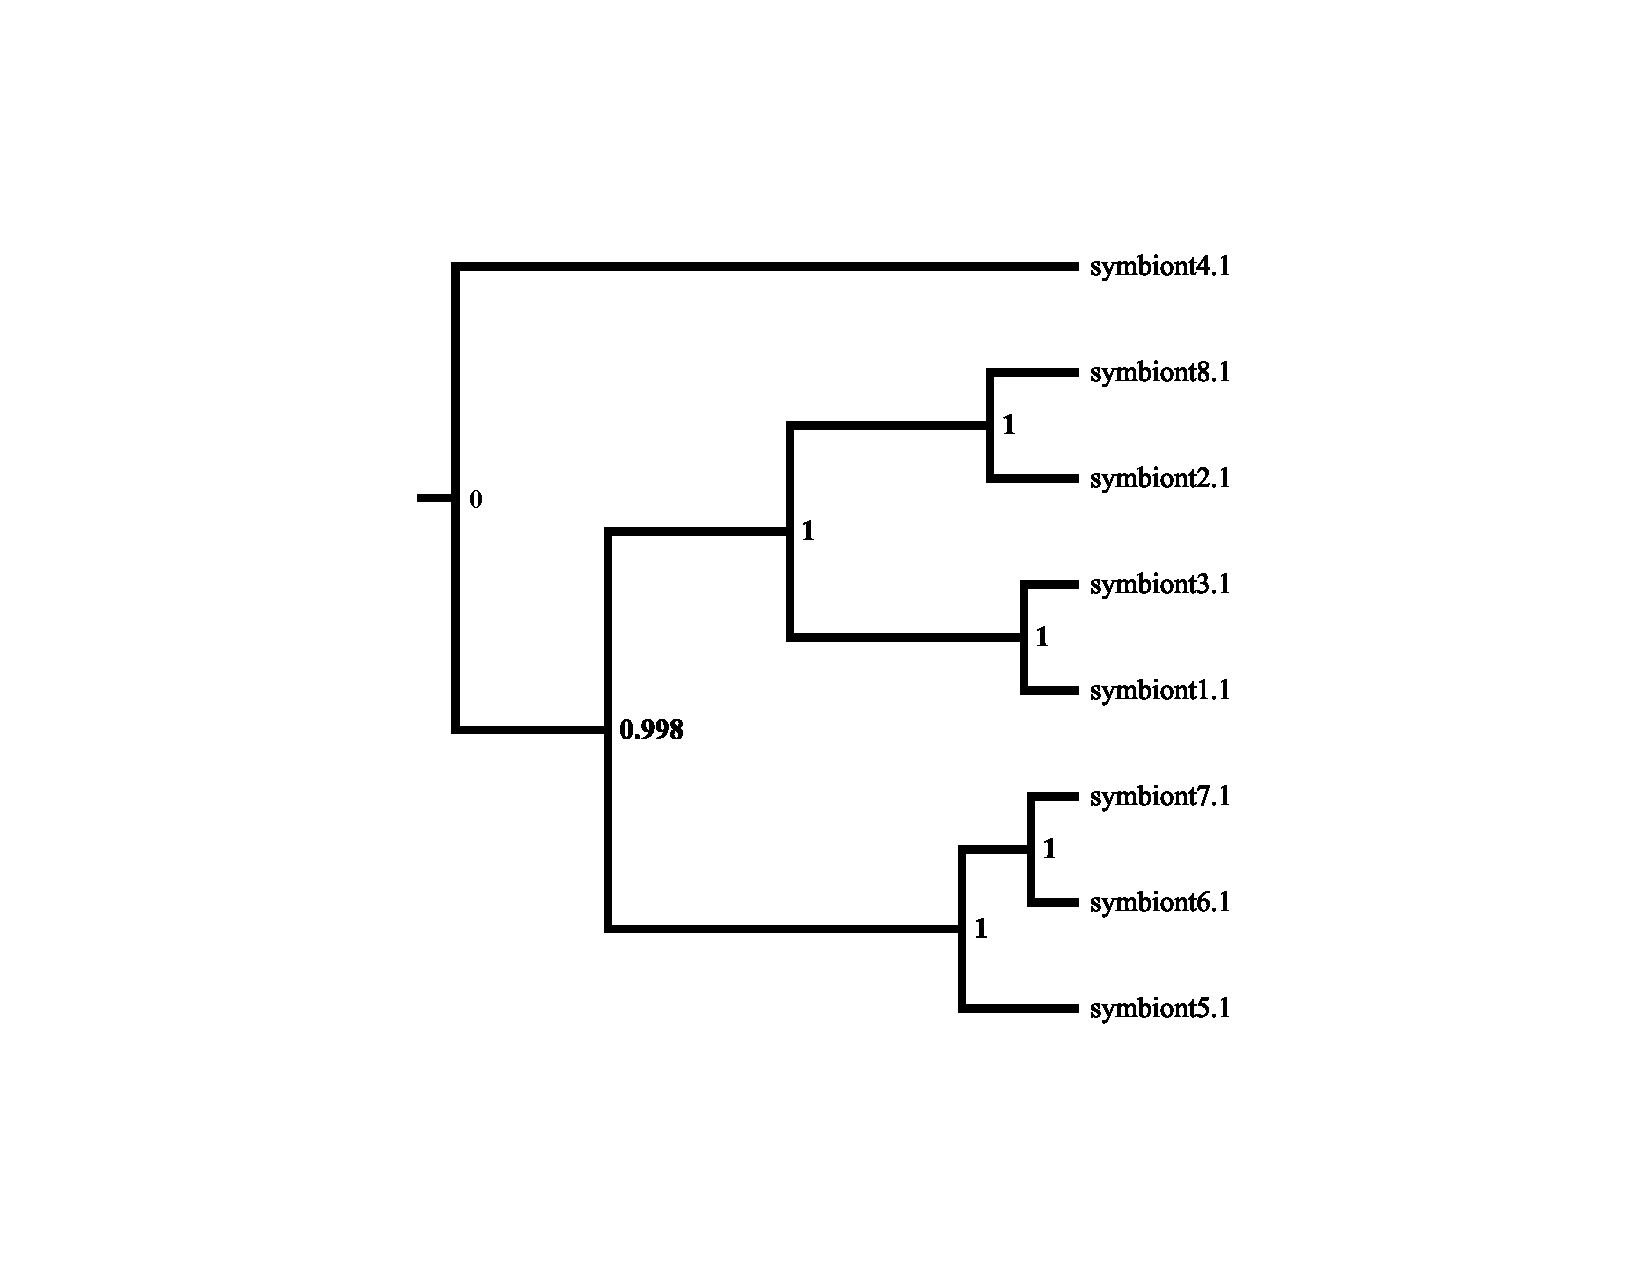
\includegraphics[width=0.5\textwidth]{figures/sim2.pdf}
\caption{The reconstructed \ac{MCC} symbiont phylogeny from simulation 1, where the values at each node represent the posterior probability that the node was reconciled to the correct host node.}
\label{fig:sim1}
\end{SCfigure}

The biggest issue with simulation 1 was the failure to recover the symbiont's host at the root, which should be the root of the host tree ($P = 0$), despite accurate recovery of the ancestral host at all other nodes of the symbiont tree ($P \approx 1$ at these nodes). In hindsight, this appears to be a shortcoming of the implemented operator. For a reconciliation to be valid ($P>0$), a symbiont and its host must be contemporaneous. To avoid proposing a state that will definitely be rejected, the host-switch operator assigns a symbiont a host that it is currently contemporaneous with (a new host which is therefore partially contemporaneous to the symbiont's current host). Because the root of a tree can never be contemporaneous with any other node in that tree, the operator can never switch a symbiont from its current host to the root of the host tree or vice versa. Thus it is impossible to transition to or from a state in which a symbiont is associated with the root under my current implementation.

\singlespacing
\begin{table}
\centering
\caption{The actual and estimated values for the \ac{MCMC} analysis of simulation 2.}
\begin{tabular}{r r r}
\toprule
\textbf{Parameter} & \textbf{Actual} & \textbf{Estimated (median)} \\
\midrule
duplication rate $\lambda$ & 1.0 & 1.419 \\
host-switch rate $\tau$ & 1.0 & 2.471 \\
loss rate $\mu$ & 1.0 & 1.606 \\
\bottomrule
\end{tabular}
\label{tab:sim2}
\end{table}
\doublespacing

\begin{SCfigure}
\centering
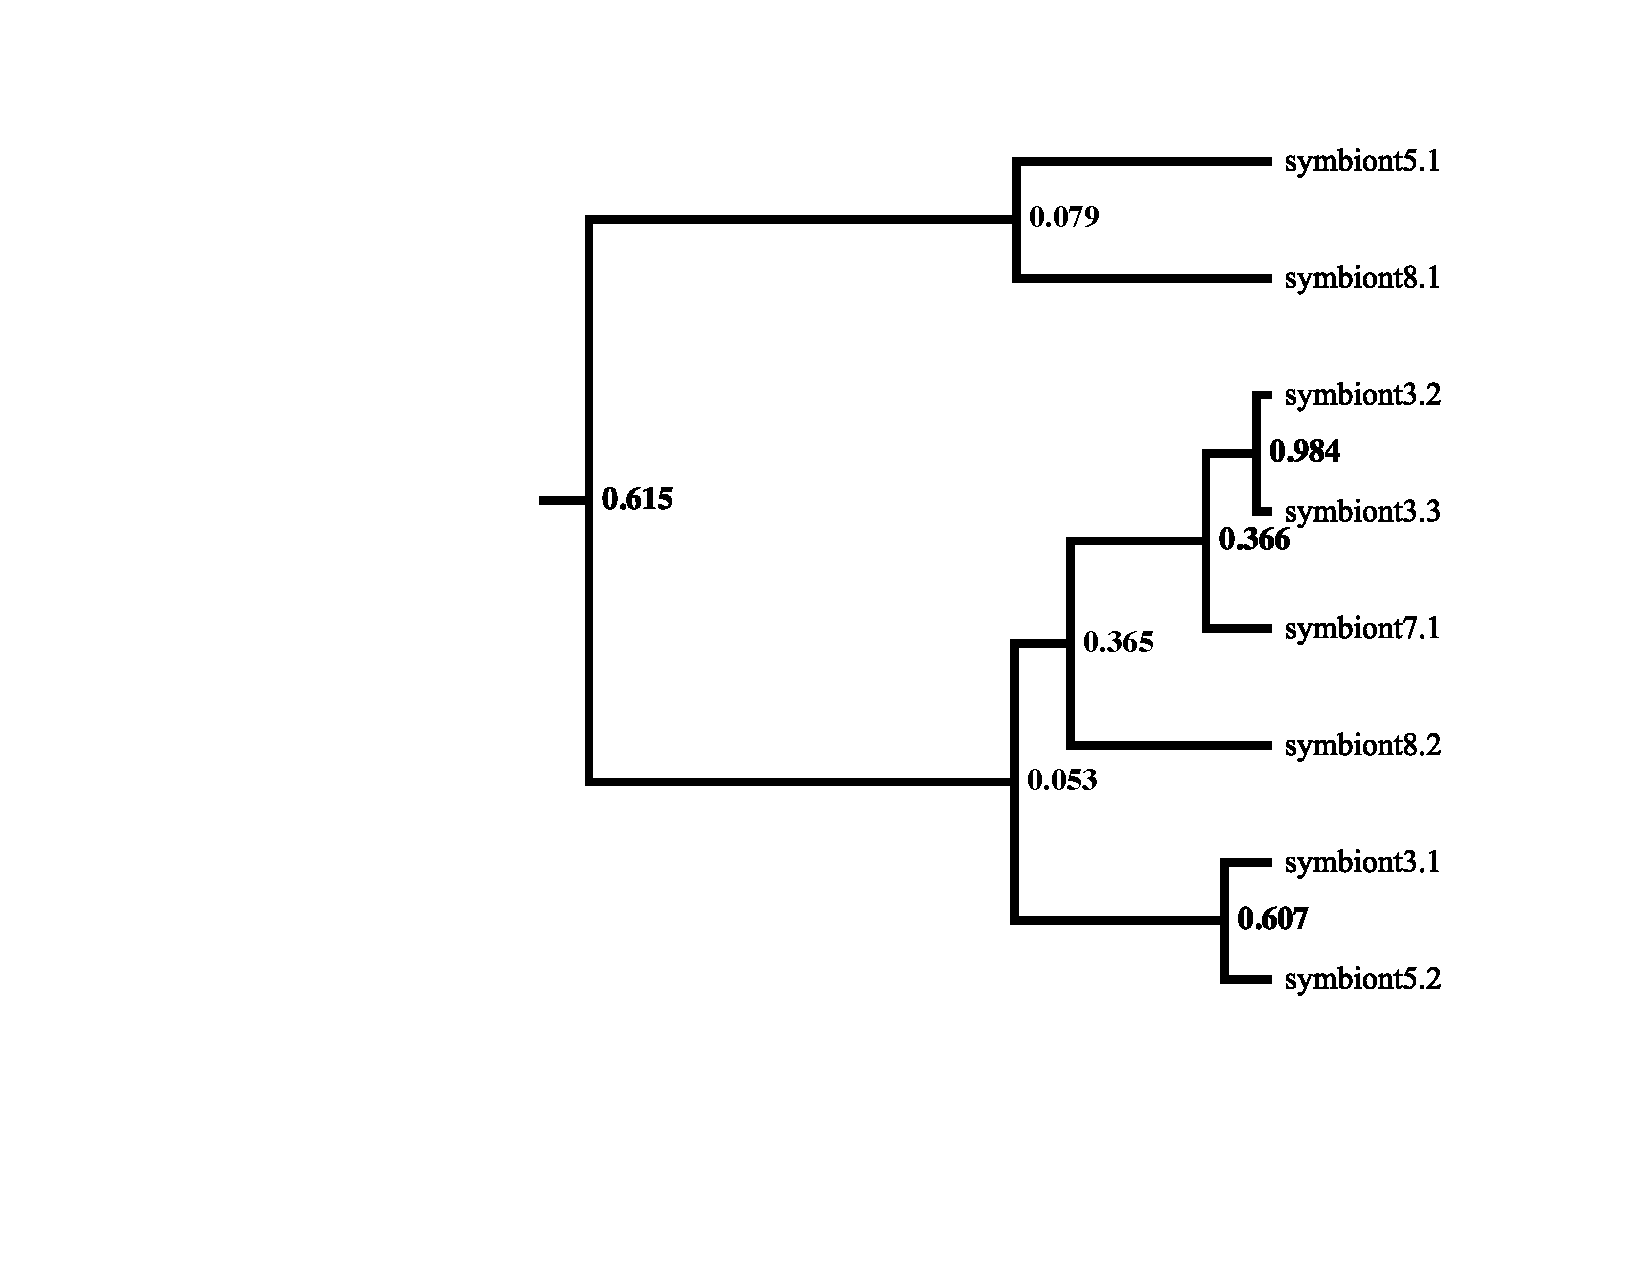
\includegraphics[width=0.5\textwidth]{figures/sim1.pdf}
\caption{The reconstructed \ac{MCC} symbiont phylogeny from simulation 2, where the values at each node represent the posterior probability that the node was reconciled to the correct host node.}
\label{fig:sim2}
\end{SCfigure}

Estimated rates from the both simulations (see Tables~1 and~2) are all significantly larger than the original rates used for simulation. Because the values are the median from an integration over all reconstructions, they are influenced by the high rates necessary to increase the likelihood complicated reconstructions that involve many host-shifts. This is a artifact of Bayesian similar in phenomenon to the long branch attraction demonstrated by \textcite{Kolaczkowski:2009}.

Although the reconstruction of simulation~1 was nearly perfect and strongly supported, due to its simple nature (Figure~5), support for the reconciliation of simulation~2 had varied support at each node (Figure~6). Only one node shows high support for its reconciliation; all others have relatively low to very low support. Because of the small simulation dataset used, these reconciliation problems may be a combined result of the lack of data and poor selection of influential prior distributions. However, the best-supported reconciliation was the true reconciliation at 4 of the 7 internal symbiont nodes, with all other states significantly less well-supported.

At this point I do not provide diagrams of the complete reconstructed coevolutionary histories, partially due to my lack of an automated procedure to produce them. The primary difficulty is developing a method to illustrate events where multiple possible scenarios have been integrated over without compromising clarity of the figure, perhaps by adopting an approach similar to that of the phylogeny visualization program DensiTree \parencite{Bouckaert:2010}.

\section*{Conclusions and Future Work}

I implement a probabilistic cophylogeny reconciliation model and use it to reconstruct complete coevolutionary histories to some degree of accuracy, demonstrating that Bayesian \ac{MCMC} methods for reconstruction of coevolutionary histories is an achievable step forward in our research on symbioses and that considering only observations in the model provides a reasonable aproximation.

An immediate issue is the inability for the and will necessitate a more sophisticated operator that adjusts the node heights of the symbiont node while changing its host. Along these lines, the effects of the cophylogeny likelihood on mixing of the \ac{MCMC} calls for serious investigation, particularly for larger cophylogenies. The influence of the prior on the event rates and final posterior distribution with relation to the size of the dataset also warrants investigation.

Finally, although much more evaluation with simulated datasets is necessary, I developed the model with the hope of eventually applying it to real data. At the time of writing, I have begun working with some real datasets, and have met some additional challenges. Primarily, finding model systems with enough data available to create well-resolved and dated phylogenies of both the host and symbiont and integrating all of this data into a single analysis proves to be a big task.

A significant effort has been put into developing and testing alternatives to the strict clock model for molecular evolution \parencites{Drummond:2006}{Drummond:2010}{Baele:2012b}, several of which have been implemented in BEAST and can be used with my cophylogeny model. A question that should be asked in a model where rates can deviate, is whether the rate at a particular symbiont node better predicted by the symbiont phylogeny or the host phylogeny? Testing these models against each other on real datasets can yield insight to these processes.

There are several avenues upon to expand the simple cophylogeny model. For example, \textcite{Charleston:2002} and \textcite{Faria:2013} both found preferential host-switching to be a phenomenon driving the evolution of viruses with their hosts. Furthermore, a model for preferential host-switching could help estimate the risk of zoonoses transferring to humans \parencite{Charleston:2009}. A parameterization of this process could be developed and included in my model. Additionally, \textcite{Yang:2010} developed a Bayesian \ac{MCMC} methodology to determine the species delimitations between a set of individuals and \textcite{Heled:2010a} implemented species tree inference in BEAST. Because coevolutionary reconstruction is very dependent on the delimitations between species, a combination of these models could be extremely informative. Finally, my cophylogeny model could also easily be expanded to support geographical data simply by restricting a given symbiont's location to that of its host and using the existing phylogeography implementations in BEAST to calculate its likelihood \parencites{Lemey:2009}{Lemey:2010}. Again, model testing could be used to evaluate specific hypotheses about these processes.

Several of these potential extensions relate directly to the \ac{GMTC}, which describes coevolution as a process that occurs when a species is partitioned into (made into a \enquote{mosaic} of) multiple, local populations, where symbiotic specialization occurs only in coevolutionary \enquote{hotspots}, or populations with low rates of incoming gene flow \parencite{Thompson:2005}. Ultimately, it may be possible to develop a model that encompasses all aspects of the \ac{GMTC}, and thus to empirically test the robustness of the \ac{GMTC} against coevolutionary histories.

\setlength\bibitemsep{12pt}
\singlespacing
\printbibliography

\end{document}
